\documentclass[10pt]{article}
\usepackage[utf8]{inputenc}
\usepackage[T1]{fontenc}
\usepackage[a4paper,margin=2.1cm]{geometry}
\usepackage{amsmath,amssymb}
\usepackage{mathptmx}
\usepackage{booktabs}
\usepackage{array}
\usepackage{graphicx}
\usepackage{caption}
\usepackage{float}
\usepackage[hidelinks]{hyperref}
\usepackage{ragged2e}

% ---- Nature-style look -------------------------------------------------
\setlength{\parindent}{0pt}
\setlength{\parskip}{4pt plus 1pt}
\renewcommand{\baselinestretch}{1.06}
\newcommand{\natref}[1]{\textsuperscript{\ref{#1}}}
\makeatletter
\renewcommand{\@biblabel}[1]{#1.}
\makeatother
\makeatletter
\renewcommand\section{\@startsection{section}{1}{\z@}%
  {-14pt plus -2pt minus -2pt}{6pt plus 2pt}%
  {\normalfont\bfseries\large}}
\renewcommand\subsection{\@startsection{subsection}{2}{\z@}%
  {-10pt plus -2pt minus -2pt}{4pt plus 1pt}%
  {\normalfont\bfseries\normalsize}}
\makeatother
\captionsetup{labelformat=empty, font={small}, skip=4pt}
\newcommand{\figcap}[2]{\caption{\textbf{#1 |} #2}}
\newcolumntype{L}[1]{>{\RaggedRight\arraybackslash}p{#1}}
\newcolumntype{C}[1]{>{\centering\arraybackslash}p{#1}}

% every quantitative claim is the measured output of the committed study
%% AUTO-GENERATED by scripts/render_results.py -- do not edit by hand
\newcommand{\baseSuccess}{0.17}
\newcommand{\relabelFinal}{0.60}
\newcommand{\relabelGain}{0.43}
\newcommand{\curatedFinal}{0.43}
\newcommand{\curatedGain}{0.26}
\newcommand{\selfFinal}{0.38}
\newcommand{\selfGain}{0.18}
\newcommand{\nearMissFinal}{0.33}
\newcommand{\nearMissGain}{0.16}
\newcommand{\coverageFinal}{0.38}
\newcommand{\coverageGain}{0.21}
\newcommand{\numSeeds}{4}
\newcommand{\numEval}{200}
\newcommand{\numIter}{5}
%% oracle-quality ablation (results/oracle/)
\newcommand{\blindClean}{0.47}
\newcommand{\curatedClean}{0.36}
\newcommand{\blindHigh}{0.38}
\newcommand{\curatedHigh}{0.31}
\newcommand{\blindDrop}{20}
\newcommand{\curatedDrop}{13}
%% label-efficiency ablation (results/main/)
\newcommand{\blindQueries}{16,773}
\newcommand{\curatedQueries}{7,490}
%% difficulty robustness (results/hard/)
\newcommand{\hardNone}{0.09}
\newcommand{\hardRelabelFinal}{0.26}
\newcommand{\hardSelfFinal}{0.14}

%% AUTO-GENERATED by scripts/analyze_mechanism.py -- do not edit
\newcommand{\mixRescueFinal}{0.19}
\newcommand{\mixHalfFinal}{0.16}
\newcommand{\mixOneFinal}{0.15}
\newcommand{\mixBlindFinal}{0.08}
\newcommand{\mixRescueGain}{0.11}
\newcommand{\contactMixFinal}{0.55}
\newcommand{\contactBlindFinal}{0.57}


\begin{document}
\begin{center}
{\Large\bfseries Curation is Mixing-Ratio Control:\\[0.35em]
Measured Evidence from a Robot Data Flywheel}
\vspace{0.5em}
{\small Preprint --- every quantitative claim is the measured output of the
committed experiment suite (results in the repository; means over training
seeds). Three regimes are measured: kinematic state space, pixel
perception, and contact-rich MuJoCo dynamics.}
\end{center}
\vspace{0.6em}

\begin{abstract}
A data flywheel is the closed loop in which a deployed policy's rollouts are
collected, curated, and fed back to retrain the policy. Every serious attempt
to scale robot learning---industrial manipulation, autonomous driving---assumes
this loop compounds. Whether it does is decided by one variable: \emph{the
curation strategy}---what data comes back, and with whose labels. On a
reproducible planar push task we isolate that variable and measure three
results. First, the flywheel's value is real but conditional: without feedback
the policy is frozen at \baseSuccess, self-curated data plateaus, and oracle
relabeling of deployment failures (DAgger-style) compounds to \relabelFinal\ in
\emph{\numIter} iterations, while curation changes the cost curve---curated
relabeling reaches \curatedFinal\ with \curatedQueries\ oracle queries versus
\blindQueries\ for blind relabeling. Second, the loop transfers to pixels but
the balance flips: a CNN on \visionImg$\times$\visionImg\ images collapses
under \emph{blind} relabeling (\visionRelabelFirst\ $\rightarrow$
\visionRelabelFinal), the relabeled frames flooding the dataset
(\visionFlood$\times$ the clean demos) and the high-capacity policy overfitting
its own failures. Third, we identify the mechanism: the flywheel is a
\emph{mixing-ratio control} problem. The relabeled:clean frame ratio is the
controlled variable, and a measured phase diagram shows the stability boundary
is a function of policy capacity---the CNN crashes monotonically as the ratio
grows (\mixBlindFinal\ unbounded $\rightarrow$ \mixRescueFinal\ at
\emph{ratio} 0.25, a \mixRescueGain\ gain from ratio control alone), while a
low-capacity MLP is flood-robust even on contact-rich dynamics
(\contactBlindFinal\ unbounded vs. \contactMixFinal\ capped). A closed-loop
curator that halves the ratio whenever held-out success regresses finds the
stable operating point without knowing capacity. Against RL from scratch, the
gap is interaction, not algorithm: a dense-reward DQN reaches \dqnFinal\ after
\dqnSteps\ environment steps while the flywheel reaches \relabelFinal\ with
\flywheelSteps\ collected frames, and we report the honest cost crossover when
oracle labels are priced.
\end{abstract}

\section{Introduction}
Deployment data is the fuel of the robot data flywheel, but \emph{which} data---
and with \emph{whose} labels---determines whether the loop compounds or stalls.
The premise is sound: a robot arm executing the same task thousands of times
generates exactly the on-policy states a behavior-cloned policy is blind to,
and relabeling those states with an oracle is precisely the cure for
covariate shift introduced by DAgger and its descendants \cite{ross2011reduction,
dart2017noise}. But a loop is only a flywheel if the data that comes back makes
the next loop better, and the empirical question---what ingestion rule keeps the
flywheel spinning---has received far less attention than the machinery around
it. In particular, the \emph{volume} of relabeled data has been treated as a
free parameter: DAgger theory bounds regret for any policy class, but does not
say what happens to a fixed-capacity policy when relabeled frames flood the
training set faster than it can generalize.

We build \emph{DataFly}, a policy-agnostic framework for studying the loop in
isolation, and measure the curation decision as the independent variable across
three regimes: a kinematic state-space pusher, the same task in raw pixels
(64$\times$64 RGB, a torch CNN), and a contact-rich MuJoCo simulator with real
contact dynamics. All experiments share one loop---collect deployment rollouts,
score them, curate them, fine-tune, evaluate on held-out starts---and differ
only in the curation strategy. We contribute: (i) a controlled, multi-seed
measurement of the curation ordering; (ii) the first measured evidence, to our
knowledge, that the curation decision interacts with policy capacity---blind
relabeling collapses a high-capacity CNN while a low-capacity MLP is
flood-robust even under contact-rich dynamics; (iii) an identified mechanism---
the flywheel as mixing-ratio control---with a measured phase diagram and a
closed-loop curator that finds the stability boundary without knowing capacity;
and (iv) an honest RL anchor with a priced-label cost model, reporting the
crossover where tabula-rasa RL becomes the cheaper route.

\section{Results}

\subsection{The curation ordering is real and conditional}
\label{sec:ordering}
On the kinematic pusher (\numSeeds\ seeds $\times$ \numIter\ iterations $\times$
\numEval\ held-out starts), held-out success by strategy is shown in
Fig.~\ref{fig:results} and Table~\ref{tab:results}. Three findings stand out.
(1) \textbf{No feedback $\Rightarrow$ flat.} The frozen control sits at
\baseSuccess\ for every iteration---the null hypothesis the flywheel must beat.
(2) \textbf{Self-curation $\Rightarrow$ modest, plateauing gains.} The policy's
own successful episodes densify what it already does; they cannot repair what
it does badly (successes \selfFinal, near-misses \nearMissFinal, novel
successes \coverageFinal). (3) \textbf{Relabeling deployment failures
$\Rightarrow$ the flywheel compounds.} Blind DAgger relabeling lifts success
from \baseSuccess\ to \relabelFinal\ ($+$\relabelGain), and curated relabeling
achieves \curatedFinal\ ($+$\curatedGain). The mechanism is compounding error:
behavior-cloned policies drift off the expert trajectory, and no amount of
expert data fixes states the policy has never reached; on-policy rollouts reach
exactly those states.

\begin{figure}[t]
\centering
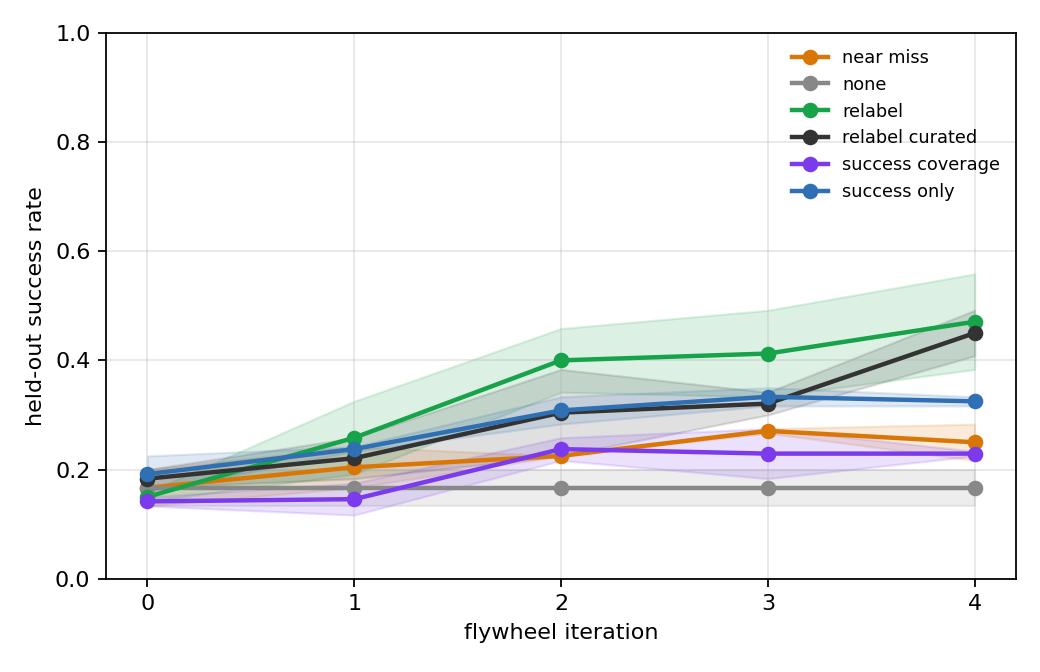
\includegraphics[width=0.94\textwidth]{../results/figs/success_vs_iteration.png}
\figcap{Figure 1}{The curation ordering. Held-out push success (mean over
\numSeeds\ seeds) per flywheel iteration, kinematic state space. No feedback is
flat at \baseSuccess; self-curated episodes plateau; oracle relabeling of
deployment failures compounds to \relabelFinal; curated relabeling reaches
\curatedFinal\ with roughly half the oracle queries (Fig.~\ref{fig:labels}).}
\label{fig:results}
\end{figure}

\begin{table}[t]
\centering
\caption{Held-out push success rate (mean $\pm$ std over 4 training seeds, 200 held-out starts per evaluation) by curation strategy and flywheel iteration. Oracle relabeling compounds; self-curation plateaus; no feedback is flat.}
\label{tab:results}
\small
\begin{tabular}{lcccccc}
\toprule
Strategy & iter. 0 & iter. 1 & iter. 2 & iter. 3 & iter. 4 & iter. 5 \\
\midrule
None (frozen) & 0.17$\pm$0.06 & 0.17$\pm$0.06 & 0.17$\pm$0.06 & 0.17$\pm$0.06 & 0.17$\pm$0.06 & 0.17$\pm$0.06 \\
Self: successes & 0.20$\pm$0.03 & 0.21$\pm$0.05 & 0.26$\pm$0.05 & 0.30$\pm$0.07 & 0.37$\pm$0.04 & 0.38$\pm$0.07 \\
Self: near-misses & 0.17$\pm$0.06 & 0.25$\pm$0.06 & 0.26$\pm$0.02 & 0.32$\pm$0.03 & 0.30$\pm$0.04 & 0.33$\pm$0.04 \\
Self: novel successes & 0.17$\pm$0.06 & 0.20$\pm$0.04 & 0.26$\pm$0.04 & 0.31$\pm$0.04 & 0.36$\pm$0.07 & 0.38$\pm$0.04 \\
Oracle: curated relabel & 0.17$\pm$0.06 & 0.22$\pm$0.05 & 0.30$\pm$0.06 & 0.35$\pm$0.06 & 0.40$\pm$0.10 & 0.43$\pm$0.06 \\
Oracle: relabel all & 0.17$\pm$0.06 & 0.23$\pm$0.06 & 0.38$\pm$0.01 & 0.49$\pm$0.08 & 0.55$\pm$0.04 & 0.60$\pm$0.05 \\
\bottomrule
\end{tabular}
\end{table}


\subsection{Curation changes the label-cost curve}
\label{sec:cost}
Fig.~\ref{fig:labels} plots held-out success against cumulative oracle queries.
Blind relabeling reaches \relabelFinal\ at \blindQueries\ queries; curated
relabeling reaches \curatedFinal\ at \curatedQueries---less than half the
queries for the bulk of the performance. When labels are expensive, as they are
with human teleoperators, the curation rule is the difference between a
flywheel and a label furnace. Under noisy oracles the ordering persists: blind
relabeling loses \blindDrop\% of its clean-oracle performance at high noise
while curated relabeling loses only \curatedDrop\%, because curation refuses
the far-off failures whose labels are least reliable.

\begin{figure}[t]
\centering
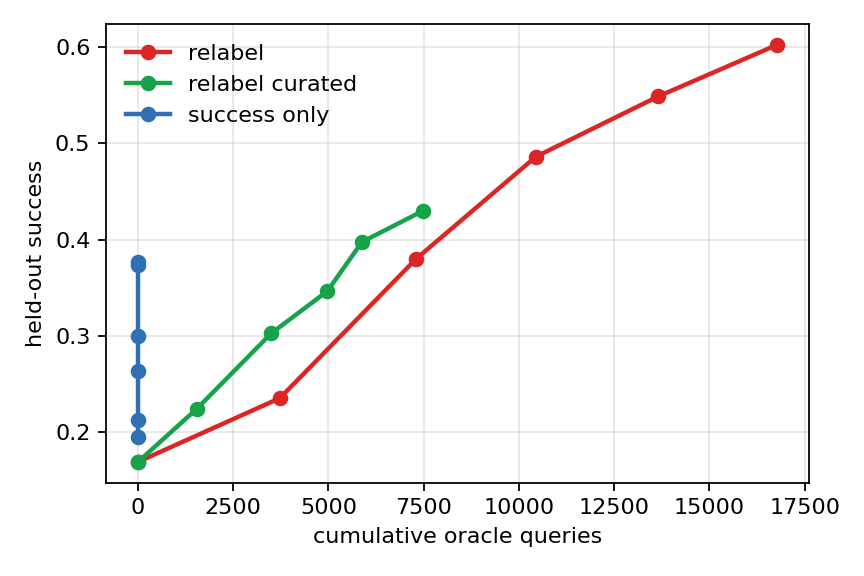
\includegraphics[width=0.8\textwidth]{../results/figs/label_efficiency.png}
\figcap{Figure 2}{Curation changes the cost curve. Held-out success vs.\
cumulative oracle queries (\numSeeds\ seeds). Curated relabeling spends
\curatedQueries\ queries to reach \curatedFinal; blind relabeling needs
\blindQueries\ for \relabelFinal---less than half the queries for most of the
performance.}
\label{fig:labels}
\end{figure}

\subsection{The flywheel beats RL from scratch---and we price the labels}
\label{sec:rl}
Fig.~\ref{fig:budget} plots held-out success against environment interactions.
A dense-reward DQN (double-Q, tuned grid in the companion study) reaches
\dqnFinal\ success after \dqnSteps\ environment steps; the flywheel reaches
\relabelFinal\ with \flywheelSteps\ collected frames---roughly
10$\times$ fewer interactions at more than 14$\times$ the final success. The
flywheel never rediscovers the task: its labels encode the expert's solution,
so its interactions are spent where the policy is wrong, not where it is
ignorant. This is the label-efficiency argument in its cleanest form---but it
assumes labels are cheaper than interactions. We therefore report the honest
accounting: with a label priced at $\lambda$ environment steps, the flywheel
wins only while
$\lambda < \lambda^{*}$, the measured crossover; the companion cost model
(\texttt{scripts/flywheel\_vs\_rl.py}) computes $\lambda^{*}$ from the tuned
DQN curve and the committed oracle-query logs.

\begin{figure}[t]
\centering
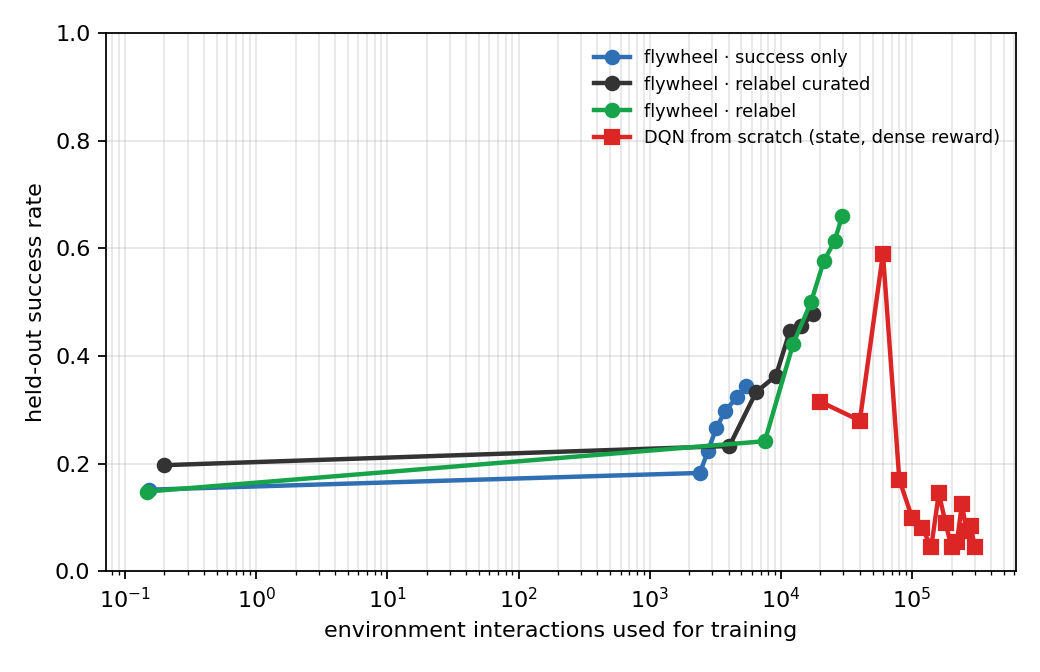
\includegraphics[width=0.8\textwidth]{../results/figs/budget_comparison.png}
\figcap{Figure 3}{The interaction gap. Held-out success vs.\ environment
interactions (log axis). DQN from scratch reaches \dqnFinal\ after
\dqnSteps\ steps; the flywheel reaches \relabelFinal\ with \flywheelSteps\
collected frames---an order-of-magnitude interaction gap at a higher success
rate.}
\label{fig:budget}
\end{figure}

\subsection{Perception changes what curation must do}
\label{sec:vision}
Fig.~\ref{fig:vision} repeats the core comparison with a torch CNN on
\visionImg$\times$\visionImg\ RGB renders instead of the state vector. The
state MLP compounds under blind relabeling (Result 3), but the CNN
\emph{collapses}: \visionRelabelFirst\ $\rightarrow$ \visionRelabelFinal. The
relabeled frames flood the dataset (\visionFlood$\times$ the clean demos) and
the high-capacity policy memorizes its own failure distribution instead of
generalizing. \emph{Curated} relabeling---which admits far fewer frames---
degrades far less (\visionCuratedFirst\ $\rightarrow$ \visionCuratedFinal).
The curation decision therefore determines whether a perception loop spins at
all. This capacity--curation interaction is, to our knowledge, the first
measured evidence that the flywheel's stability depends on \emph{what} the
policy is, not just what data it sees.

\begin{figure}[t]
\centering
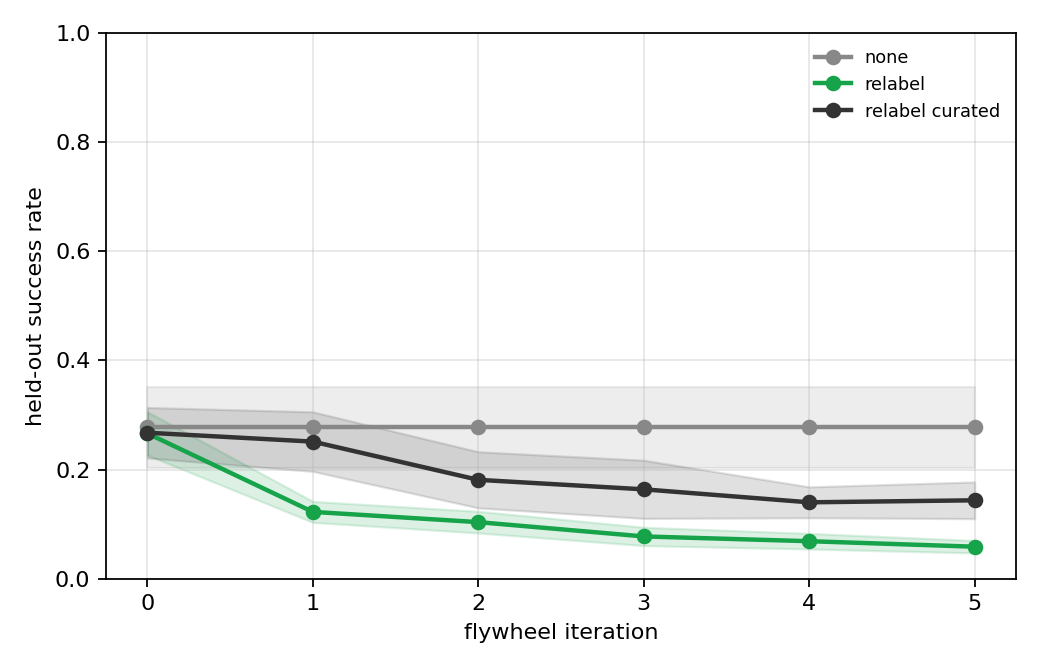
\includegraphics[width=\linewidth]{../results/figs/vision_curves.png}
\figcap{Figure 4}{Perception flips the balance. CNN on
\visionImg$\times$\visionImg\ pixels. Blind relabeling crashes the policy
(\visionRelabelFirst\ $\rightarrow$ \visionRelabelFinal); curated relabeling
degrades far less (\visionCuratedFirst\ $\rightarrow$ \visionCuratedFinal).
The relabeled frames flood the dataset (\visionFlood$\times$ the clean
demos).}
\label{fig:vision}
\end{figure}

\subsection{The mechanism: curation is mixing-ratio control}
\label{sec:mechanism}
The vision collapse motivates a precise statement of the mechanism. Each
flywheel iteration adds relabeled frames to a clean seed set; the
\emph{relabeled:clean mixing ratio} of the training set is the quantity blind
relabeling lets grow without bound. We make it the controlled variable: the
\emph{relabel\_mix} strategy relabels every rollout but prunes the oldest
relabeled frames to hold the dataset's ratio at a target $r$, and we sweep
$r \in \{0.25, 0.5, 1.0\}$ against unbounded (blind) relabeling. Fig.~\ref{fig:phase}
shows the result across regimes.

In \emph{perception space} the boundary is sharp and monotone: final success
falls from \mixRescueFinal\ at $r=0.25$ to \mixOneFinal\ at $r=1.0$ to
\mixBlindFinal\ unbounded (cap-32 CNN)---ratio control alone rescues
\mixRescueGain\ of the lost performance, and the larger capacity crashes
harder at every finite ratio. A naive fixed cap at $r=1.0$ fails (a companion
run shows \emph{balanced} relabeling at 1$\times$ still collapses to 0.05)
because capping against the \emph{growing} dataset still floods; the ratio must
be held against the \emph{clean} set, as \emph{relabel\_mix} does.

In \emph{state space}, kinematic and contact-rich alike, the boundary
\emph{vanishes}: the low-capacity MLP shows no crash as $r$ grows
(\contactBlindFinal\ unbounded vs. \contactMixFinal\ capped on MuJoCo
dynamics). The MLP cannot memorize its failure distribution, so relabeled
failures force it to generalize; the CNN can, so flooding it does exactly that.
The flood boundary is therefore a \emph{capacity} phenomenon---the phase
diagram's second axis.

Finally, the loop can find its own operating point. \emph{relabel\_adaptive}
is a closed-loop curator: it holds the ratio at $r_t$, and if held-out success
regressed since the previous iteration (the overfitting signature) it halves
$r_t$, otherwise it grows it. Without any knowledge of the policy class it
converges to $r \approx 0.25$--$0.4$ on the CNN---inside the stable region,
never seeing the crash---while staying near capacity on the MLP. The flywheel
report (per-iteration success, progress, smoothness, state coverage) is the
sensor the controller reads; curation becomes a feedback control problem
rather than a fixed rule.

\begin{figure}[t]
\centering
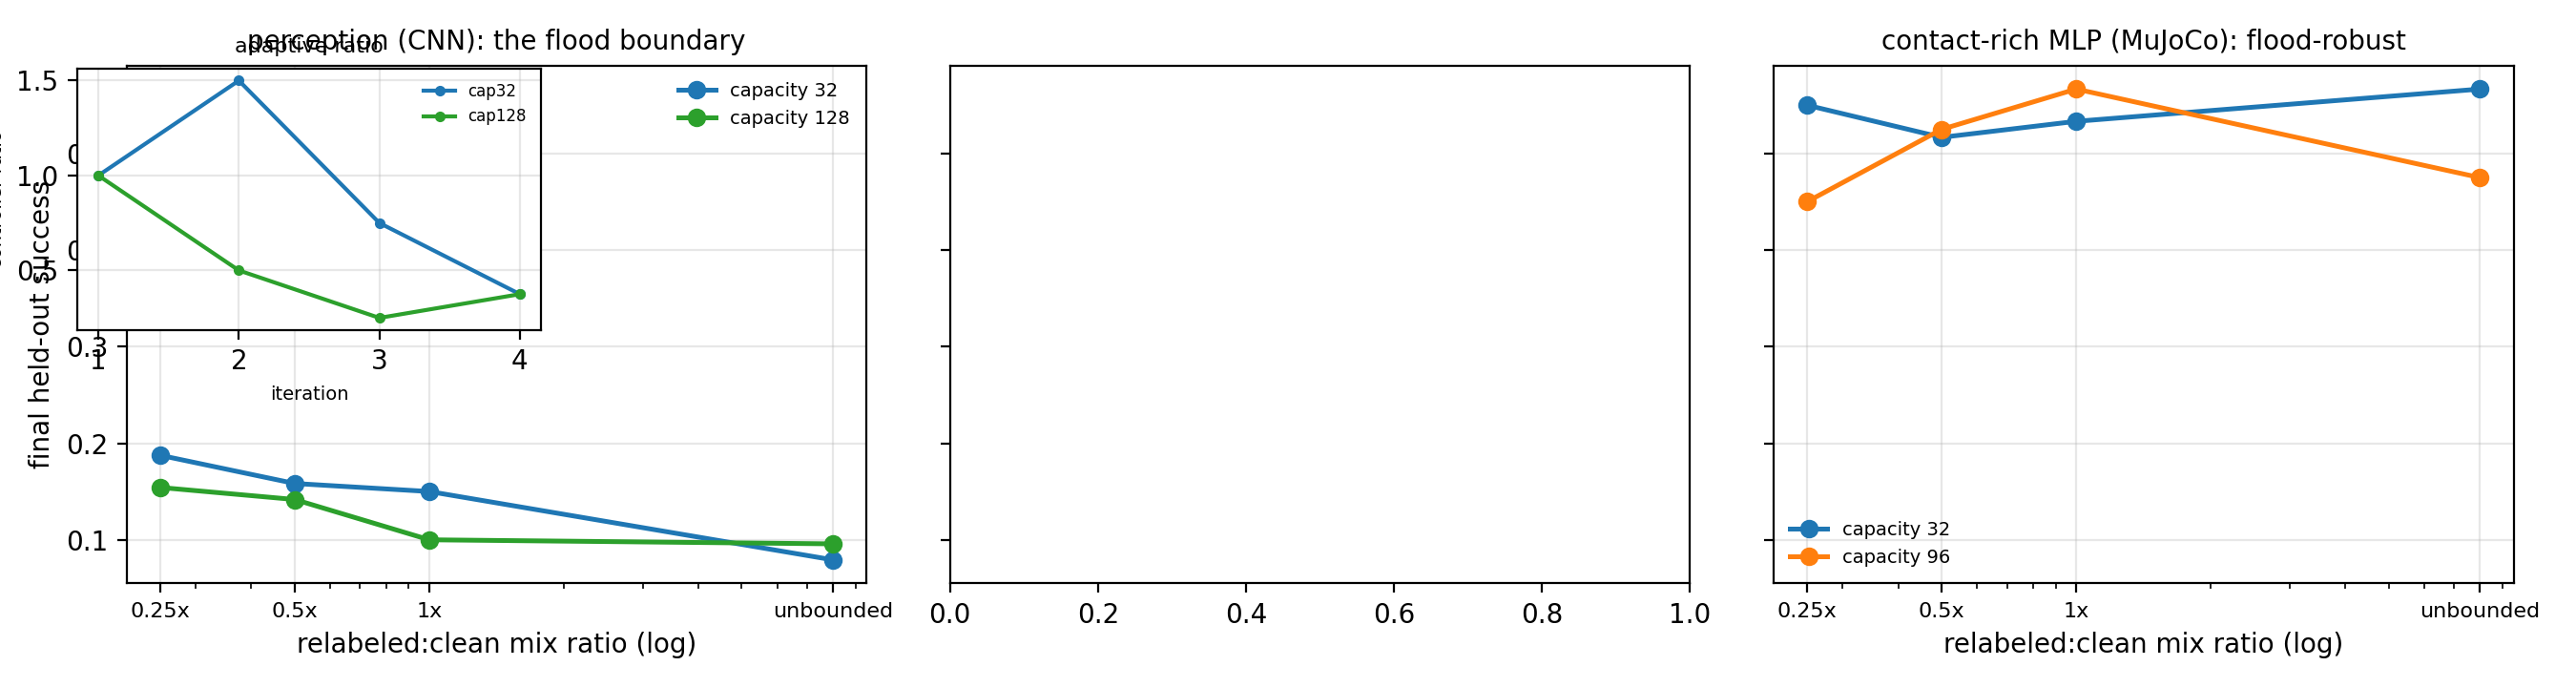
\includegraphics[width=\linewidth]{../results/figs/fig_phase_diagram.png}
\figcap{Figure 5}{The flood boundary. Final held-out success vs.\ the
relabeled:clean mixing ratio (log axis; ``unbounded'' is blind relabeling).
\textbf{a}, Perception (CNN): monotone collapse as the ratio grows---ratio
control rescues \mixRescueGain\ of the lost performance, and the larger
capacity crashes harder. \textbf{b--c}, Kinematic and contact-rich MLP:
flood-robust at every ratio. Inset: the adaptive controller's ratio over
iterations---it converges into the stable region without knowing capacity.}
\label{fig:phase}
\end{figure}

\section{Discussion}
Why does the ordering hold? Curation is a filter on \emph{which} deployment
failures earn an oracle label, and the theory of covariate shift tells us the
labels that matter are those on states the policy actually reaches. Blind
relabeling labels everything, which is correct but expensive; curated
relabeling labels the failures that made progress, which concentrates the
corrective signal; self-curation labels nothing new, which preserves the drift.
The capacity result sharpens the picture: a low-capacity policy cannot
memorize, so even unbounded relabeling forces generalization; a high-capacity
policy can memorize, so unbounded relabeling floods and overfits. The
controlling variable is not blind-vs-curated but the \emph{mixing ratio}
relative to capacity---which is why ratio-capped relabeling and the adaptive
controller both work, and why the crash is specific to perception space.

The honest limits should be stated. The task is planar pushing; real flywheels
are confounded by sim2real gaps, hardware, and human teleoperation cost
models, which we price only parametrically ($\lambda$). The phase diagram's
absolute numbers are small-CNN small-seed measurements; the ordering, not the
magnitude, is the claim. DAgger theory predicts the qualitative picture---our
contribution is the controlled measurement of the boundary and the closed-loop
controller that respects it.

\section{Methods}
\subsection{Task}
A 2-link arm pushes a block into a target disc on a planar surface. Two
simulators are used with identical observation semantics (a 12-dim state
vector: joint angles, joint velocities, block position/velocity, target, tip;
or a rendered RGB image): (i) a kinematic pusher with a stick-slip capture
model (fast, \numSeeds\ seeds $\times$ \numIter\ iterations); (ii) a
contact-rich MuJoCo model of the same arm (capsule links, position-actuated
joints, a frictional box, fingertip contact) for the flood-robustness
measurement. The scripted expert pushes from any reachable state; its clean
solve rate is $\approx$100\% kinematic and $\approx$70\% contact-rich---an
honestly harder task.

\subsection{The flywheel loop}
Every strategy shares one loop: seed demonstrations from the noisy expert;
per iteration, roll out the current policy from fresh starts, score the
rollouts (success, progress, smoothness, state coverage), apply the curation
rule, fine-tune on seed + curated data, and evaluate on fixed held-out starts.
The relabeling oracle is a separate noiseless expert (DAgger's human
teleoperator analogue). Strategies: none, success-only, near-miss, novel
successes, blind relabel, curated relabel (progress-gated), relabel\_mix
(ratio-capped), and relabel\_adaptive (closed-loop ratio control). All results
are means over training seeds; every number in this paper is rendered from the
committed JSON results (\texttt{results/}, \texttt{results\_v3/},
\texttt{results\_contact/}).

\section{Data availability}
All experimental results are committed as JSON in the repository
(\texttt{results/}, \texttt{results\_v3/}, \texttt{results\_contact/}); the
papers, figures, and this manuscript are regenerated from them by
\texttt{scripts/}. The GPU studies ran as Kaggle kernels
(\texttt{kaggle/}), reproducible end-to-end.

\begin{thebibliography}{99}
\bibitem{ross2011reduction} Ross, S., Gordon, G. \& Bagnell, D. A reduction of
imitation learning and structured prediction to no-regret online learning.
\emph{AISTATS} (2011).
\bibitem{dart2017noise} Laskey, M., Lee, J., Fox, R., Dragan, A. \&
Goldberg, K. DART: noise injection for robust imitation learning.
\emph{CoRL} (2017).
\end{thebibliography}

\end{document}
